\documentclass{beamer}
\usetheme{metropolis}
%\setbeamersize{text margin left=.2cm,text margin right=.2cm}
\usepackage{graphicx}
\graphicspath{{../../images/}}
%\usepackage[french]{babel}
%\usepackage{listings}
%\usepackage{lipsum}
\usepackage{boolexpr}
\usepackage{kpfonts}
\usepackage{caption}
\usepackage{wrapfig}
%\usepackage{chngcntr}
\usepackage[labelformat=empty]{caption}
\usepackage[official]{eurosym}

\usepackage{minted}

\usepackage{siunitx}

% http://tex.stackexchange.com/questions/114830/how-can-i-use-lvert-and-rvert-norm-symbols-x-with-the-iwona-math-font
\usepackage[math]{iwona}
\usepackage{scalerel}
\def\lVert{\mid\!\mid}
\def\rVert{\mid\!\mid}

\usepackage[normalem]{ulem}
%\newcommand{\Adj}{\mathbf{A}}
\usepackage{mathtools}

\usepackage{../../custom}
\usepackage{amsfonts}
%\newcommand{\jsrcodepath}{../../code}
%\usepackage{jsr}

\newcommand{\expe}[2]{\la #1, #2 \ra}

\usepackage{framed}

%\usepackage{mathtools,xparse}
%\DeclarePairedDelimiter{\norm}{\lVert}{\rVert}
\newcommand\Wider[2][3em]{%
\makebox[\linewidth][c]{%
  \begin{minipage}{\dimexpr\textwidth+#1\relax}
  \raggedright#2
  \end{minipage}%
  }%
}

\newcommand{\aeur}{\alpha_\text{\euro}}
\newcommand{\adol}{\alpha_\$}
\newcommand{\apou}{\alpha_\text{\pounds}}

\title{Symmetry reduction for Sum-of-Squares programming}
\date{July, 2021}
\author{Beno\^it Legat \and Marek Kaluba \and Tillmann Weisser}
\institute{JuliaCon 2021}
%\institute{UCLouvain\\
%           Massachusetts Institute of Technology (MIT)\\
%           Rice University\\
%           Los Alamos National Laboratory (LANL)}

% https://tex.stackexchange.com/questions/426088/texlive-pretest-2018-beamer-and-subfig-collide
\makeatletter
\let\@@magyar@captionfix\relax
\makeatother
\begin{document}
  \maketitle

  \begin{frame}{Nonnegative polynomial into sum of squares}
  \begin{tikzpicture}
    \draw[->, bend left=20] (.6, 1.6) node[above] {$(x^3, x^2, x)$} to (.9, 1.35);
    \draw[->, bend right=30] (2.1, 2) node[right] {\alert{\emph{not} unique}} to (1.55, 1.35);
    \node at (-.1, 1.2) {$p(x)$};
    \node at (.5, 1.2) {$=$};
    \node at (1.3, 1.2) {$X^\Tr Q X$};
    \node at (-1.5, 0) {$x^6 - 2x^4 + 2x^2$};
    \node at (.5, 0) {$=$};
    \node at (2.4, 0) {$X^\Tr \begin{pmatrix}1 & 0 & -1\\\cdot & 0 & 0\\ \cdot & \cdot & 2\end{pmatrix} X$};
    \node at (-1, -1.5) {$p(x) \geq 0$ $\forall x$};
    \node at (1.5, -1.5) {$Q \succeq 0$};
    \node at (.5, -1.5) {$\Longleftarrow$};
    \draw[->] (2.5, -1) to node[right] {cholesky} (2.5, -2.5);
    \node at (-2.2, -3.5) {$x^2 + (-x^3 + x)^2$};
    \draw[->] (.2, -3.5) to (-.6, -3.5);
    \node at (3.3, -3.5) {$X^\Tr \begin{pmatrix}0 & 0 & 1\\-1 & 0 & 1\end{pmatrix}^\Tr \begin{pmatrix}0 & 0 & 1\\-1 & 0 & 1\end{pmatrix} X$};
  \end{tikzpicture}

      \noindent {\tiny Gatermann, Parrilo, \emph{{S}ymmetry groups, semidefinite programs, and sums of squares}, Journal of Pure and Applied Algebra, 2004: Example~5.1}
\end{frame}

\begin{frame}{Semidefinite program}
%  \begin{columns}
    %\begin{column}{0.48\textwidth}
      \begin{equation*}
        \label{eq:sdp_standard}
        \begin{array}{rl}
          \min\limits_{X \in \SymK[N]} & \la C, Q \ra\\
          \text{subject to:} & \la A_i, Q \ra = b_i, \quad i=1,2,\ldots,m\\
          & Q \succeq 0.
        \end{array}
      \end{equation*}
    %\end{column}
    %\begin{column}{0.48\textwidth}
      Is $x^6 - 2x^4 + 2x^2$ a sum of squares ?
      $$
      X =
      \begin{bmatrix}
        x^3\\
        x^2\\
        x
      \end{bmatrix},
      XX^\Tr =
      \begin{bmatrix}
        x^6 & x^5 & x^4\\
        \cdot & x^4 & x^3\\
        \cdot & \cdot & x^2
      \end{bmatrix},
      A_{x^6} =
      \begin{bmatrix}
        1 & 0 & 0\\
        \cdot & 0 & 0\\
        \cdot & \cdot & 0
      \end{bmatrix},
      A_{x^5} =
      \begin{bmatrix}
        0 & 1 & 0\\
        \cdot & 0 & 0\\
        \cdot & \cdot & 0
      \end{bmatrix},
      $$
      $$
      A_{x^4} =
      \begin{bmatrix}
        0 & 0 & 1\\
        \cdot & 1 & 0\\
        \cdot & \cdot & 0
      \end{bmatrix},
      A_{x^3} =
      \begin{bmatrix}
        0 & 0 & 0\\
        \cdot & 0 & 1\\
        \cdot & \cdot & 0
      \end{bmatrix},
      A_{x^2} =
      \begin{bmatrix}
        0 & 0 & 0\\
        \cdot & 0 & 0\\
        \cdot & \cdot & 1
      \end{bmatrix}.
      $$
    %\end{column}
%  \end{columns}

      \noindent {\tiny Gatermann, Parrilo, \emph{{S}ymmetry groups, semidefinite programs, and sums of squares}, Journal of Pure and Applied Algebra, 2004: Example~5.1}
\end{frame}

\begin{frame}{SDP solvers}
  For $n$-variate polynomial of degree $2d$:
  $N = {n + d \choose n}, m = {n + 2d \choose n}$.
  \begin{block}{Complexity of second order interior point solvers}
    CSDP, DSDP, MOSEK, SDPA, SDPT3, SeDuMi

    Time:
    $\bigoh((mN + m^2)N^{5/2}\log(\varepsilon))$.
    Space:
    $\bigoh(m^2)$.
  \end{block}
  Too much space needed for large scale problems, alternatives:
  \begin{itemize}
  %\begin{block}{First order methods}
    \item
    Newton conjugate gradient (Newton-CG), e.g., SDPNAL.
    \item
    ADMM, e.g., CDCS, COSMO, SCS.
  %\end{block}
  %\begin{block}{Low rank methods}
    \item
    Barvinok-Pataki bound: $\exists Q$ of rank $r \le \sqrt{2m}$.
  \begin{itemize}
    \item
    Burer-Monteiro method: $Q = UU^\Tr$, $U \in \R^{N \times r}$, e.g. SDPLR.
    \item
    Primal-dual hybrid gradient (PDHG), e.g., ProxSDP.
  \end{itemize}
  \end{itemize}
  %\end{block}
\end{frame}

\begin{frame}{Schur lemma}
  \noindent$(X_i)_i\subseteq \R^{n \times n}$ \emph{reducible} if $\exists \{0\} \subset \mathcal{V} \subseteq \R^n$ s.t. $\forall i, X_i \mathcal{V} \subseteq \mathcal{V}$

  \noindent$(X_i)_i\subseteq \R^{n \times n}$ \emph{equivalent} to $(Y_i)_i\subseteq \R^{n \times n}$ if $\exists T$ s.t. $X_i = TY_iT^{-1}$

  If $X, Y$ are irreducible and inequivalent, then
  $$
  %\begin{bmatrix}
  %  Q_{11} & Q_{12}\\
  %  Q_{21} & Q_{22}
  %\end{bmatrix}
  Q
  \begin{bmatrix}
    X & 0\\
    0 & Y
  \end{bmatrix}
    =
  \begin{bmatrix}
    X & 0\\
    0 & Y
  \end{bmatrix}
  Q
  %\begin{bmatrix}
  %  Q_{11} & Q_{12}\\
  %  Q_{21} & Q_{22}
  %\end{bmatrix}
  %\quad
  \Rightarrow
  %\quad
  \exists c_1, c_2 \text{ s.t. }
  Q =
  \begin{bmatrix}
    c_1 I & 0\\
    0 & c_2 I
  \end{bmatrix}
   %Q_{11} = q_1 I, Q_{22} = q_2 I,
   %Q_{21} = Q_{12} = 0.
  $$

  If $X$ is irreducible, then (permuting rows/columns give
  $I \otimes C$)
  $$
  %\begin{bmatrix}
  %  Q_{11} & Q_{12}\\
  %  Q_{21} & Q_{22}
  %\end{bmatrix}
  Q
  \begin{bmatrix}
    X & 0\\
    0 & X
  \end{bmatrix}
    =
  \begin{bmatrix}
    X & 0\\
    0 & X
  \end{bmatrix}
  Q
  %\begin{bmatrix}
  %  Q_{11} & Q_{12}\\
  %  Q_{21} & Q_{22}
  %\end{bmatrix}
  %\quad
  \Rightarrow
  %\quad
  \exists C \in \SymK \text{ s.t. }
  Q = C \otimes I =
  \begin{bmatrix}
    c_{1,1}I & c_{1,2}I\\
    c_{1,2}I & c_{2,2}I
  \end{bmatrix}
   %Q_{11} = q_1 I, Q_{22} = q_2 I,
   %Q_{21} = Q_{12} = 0.
  $$

  \noindent {\tiny Sagan, \emph{The symmetric group}, Springer Science \& Business Media, 2001: Definition~1.4.5, Definition~1.6.2, Example~1.7.2, Example~1.7.3 (adapted from $\mathcal{C}^{n \times n}$ to symmetric matrices $\SymK \subseteq \mathcal{R}^{n \times n}$)}
\end{frame}

\begin{frame}[fragile]
  \frametitle{SDP solvers}
  \begin{minted}{Julia}
    using SumOfSquares
  \end{minted}
\end{frame}

  \begin{frame}{Group Theory to the rescue!}
  \begin{block}{Definition}
    A \alert{group} $(G, *)$ is a set closed under the multiplication $*$, together with the existence of unique inverse elements.
  \end{block}
    {\small Example: The set of all bijections of the set $\{1,\ldots n\}$ with composition is a group (known as the full symmetric group on $n$ letters $S_n$).}

    $S_2 = \{(1)(2), (1,2)\}$ \alert{acts} on polynomial ring $\mathbb{R}[x]$ by
    \begin{align*}
      ((1)(2), x) & \mapsto x\\
      ((1, 2), x) & \mapsto -x.
    \end{align*}
    {\small 
%     Observe: $f(x) = x^4 - 2x^2$ is invariant under this action.\\
    Observe: $f(x) = x^6 - 2x^4 + 2x^2 = x^2 + (x-x^3)^2$ is invariant, but $x-x^3$ isn't!}

\end{frame}


\begin{frame}{Isotypical projections}
    ``Types'' of actions $\leftrightarrow$  blocks in the block-diagonalization:
    \[V \cong V_1 \oplus \cdots \oplus V_k.\]
    Each block $V_i$ decomposes further as
    $V = \bigoplus_i \oplus_{m_i} V_i'$. (\footnote{$m_i$ is the multiplicity of the action type in $V$})

    Universal (baseless) \alert{projections}\footnote{related to irreducible characters} in group ring $\mathbb{R}[G]$ $\leftrightarrow$ projections onto blocks (for every representation $V$!).
%
    \begin{block}{Example}
    \small
    Universal \textbf{projections} for $S_2$:\\[-0.2in]
    \begin{align*}
      \pi_1 = \frac{1}{2}((1)(2) + (1,2)) & \to\text{invariants}\\
      \pi_2 = \frac{1}{2}((1)(2) - (1,2)) & \to\text{flipped}
    \end{align*}
    \end{block}

\end{frame}

\begin{frame}[fragile]{Permutation symmetry example}
\footnotesize
\begin{minted}{julia}
  using PermutationGroups
  G = PermGroup([perm"(1,2,3,4)"])
  # permutation group generated by one element (cyclic of order 4)
  using DynamicPolynomials
  @polyvar x[1:4]
  poly = sum(x) + sum(x.^2)
  basis = monomials(x, 0:(maxdegree(f)÷2))
  using SymbolicWedderburn
  symmetry_adapted_basis(G, basis, Symmetry.VariablePermutation())
  # G acts by permuting variables
\end{minted}

Isotypical blocks when acting on $[1, x_1, x_2, x_3, x_4, x_5]$:
\[
  B_1 = \begin{bmatrix}
          1\\
          x_1 + x_2 + x_3 + x_4
        \end{bmatrix}
  \qquad
  B_2 = \begin{bmatrix}
          x_1 - x_3\\
          x_2 - x_4
        \end{bmatrix}
  \qquad
  B_3 = \begin{bmatrix}
          x_1 - x_2 + x_3 - x_4
        \end{bmatrix}
\]

  \[V \cong (V_{\alert{1}}' \oplus V_{\alert{1}}') \oplus V_2' \oplus V_3', \qquad d_2 = m_1 = 2, \quad d_1 = d_3 = m_2 = m_3 = 1.\]
  %\[V \cong (V_1' \oplus V_1') \oplus V_2' \oplus V_3', \qquad m_1 = 2, \quad m_2 = m_3 = 1.\]
\end{frame}

\begin{frame}[fragile]{Permutation symmetry example}
\footnotesize
\begin{minted}{julia}
  using SumOfSquares
  import ECOS # Note: ECOS doesn't support PSD cone,
  # but 2×2 psd constraints translate to SOC/quadratic constraints
  model = Model(ECOS.Optimizer)
  @variable(model, t)
  @objective(model, Max, t)
  pattern = Symmetry.Pattern(G, Symmetry.VariablePermutation())
  @constraint(model, poly - t in SOSCone(), symmetry = pattern)
  optimize!(model)
\end{minted}

\normalsize

  Naive: 15 vars 15 constrs, $Q$ is $5\times 5$; Symmetry: 5 vars 5 constrs,
  \[ Q = Q_1 \oplus (Q_{\alert{2}} \oplus Q_{\alert{2}}) \oplus Q_3 \qquad Q_1 \text{ is }2\times 2, Q_2 \text{ is }1\times 1, Q_3 \text{ is }1\times 1 \]
  %\[ m_1 \times m_1, m_2 \times m_2, m_3 \times m_3 \qquad 2\times 2, 1\times 1, 1\times 1 \]

  Note inversion: multiplicities $\leftrightarrow$ dimensions
  \[V \cong (V_{\alert{1}}' \oplus V_{\alert{1}}') \oplus V_2' \oplus V_3', \qquad d_2 = m_1 = 2, \quad d_1 = d_3 = m_2 = m_3 = 1.\]
%Note: the sizes here correspond to the multiplicities of irreducible subspaces, \textbf{not} their dimensions!

\end{frame}

\begin{frame}[fragile]{Even symmetry example\citefoot{\gatpar{}: Example~5.1}}
\footnotesize
\begin{minted}{julia}
  struct OnSign <: Symmetry.OnMonomials end
  # <: SymbolicWedderburn.Action, corresponds to x → -x
  SymbolicWedderburn.action(::OnSign, p::Permutation,
      mono::AbstractMonomial) = sign(p)^degree(mono)*mono
  G = PermGroup([perm"(1,2)"])
  @polyvar x
  f = x^6 - 2x^4 + 2x^2
  basis = monomials(x, 0:(maxdegree(f)÷2))
  symmetry_adapted_basis(G, basis, OnSign())
\end{minted}

  Isotypical blocks when acting on $[1, x, x^2, x^3]$:
\[
  B_1 = \begin{bmatrix}
          1\\
          x^2
        \end{bmatrix}
  \qquad
  B_2 = \begin{bmatrix}
          x\\
          x^3
        \end{bmatrix}
  \qquad
  V = (V_1' \oplus V_1') \oplus (V_2' \oplus V_2')
\]

  \vspace{-1em}

Naive formulation $4\times 4$-psd; with symmetry: $2\times 2$, $2\times 2$-psd.
\end{frame}

\begin{frame}[fragile]{Dihedral symmetry example\citefoot{\gatpar{}: Example~5.4}}
\footnotesize
  \begin{minted}{julia}
  @polyvar x y
  f = x^6 + y^6 - x^4 * y^2 - y^4 * x^2 - x^4 - y^4 -
      x^2 - y^2 + 3x^2 * y^2 + 1
  struct DihedralAction <:
      SymbolicWedderburn.ByLinearTransformation end
  \end{minted}
  The action is a mixture of changing sign and permuting variables.

  \vspace{-2em}

  \begin{align*}
    B_1 = [x^2 + y^2, 1], & \qquad m_1 = 2, d_1 = 1,\\
    B_2 = [x^3, x^2y, xy^2, y^3, x, y], & \qquad m_2 = 3, d_2 = 2,\\
    B_3 = [xy], & \qquad m_3 = d_3 = 1,\\
    B_4 = [x^2 - y^2], & \qquad m_4 = d_4 = 1,
  \end{align*}

  \vspace{-1em}

  $10 \times 10$-psd into $2 \times 2$, $3 \times 3$, $1 \times 1$, $1 \times 1$-psd.

  \vspace{-1em}

  \alert{Non}-commutative groups allow $d_i > 1$ $\to$ \alert{better} for the symmetrization!
\end{frame}

\begin{frame}[fragile]{Implementing group action}
\footnotesize

  \begin{minted}{julia}
  import GroupsCore
  struct DihedralGroup <: GroupsCore.Group ... end
  struct DihedralElement <: GroupsCore.GroupElement
      ...
  end
  \end{minted}
\normalsize
  \begin{itemize}
    \item implement methods from \texttt{GroupsCore.jl} API for \texttt{DihedralGroup}
    \item implement action methods from \texttt{SymbolicWedderburn} for \texttt{DihedralAction}
  \end{itemize}
\end{frame}

\begin{frame}{Behind the scenes: \texttt{SymbolicWedderburn.jl}}
    \begin{itemize}
      \item compute \alert{character table} of the group $\longrightarrow$ universal projections
      \item given action e.g. on monomials, \alert{induce} the action to the whole basis
      \item evaluate the projections in the action $\longrightarrow$ \alert{block diagonalizing} change of basis
      \item further \alert{decompose} each block into \alert{irreducible} blocks(\footnote{for now numerically only}).
    \end{itemize}
\end{frame}


\begin{frame}{Large scale example}

  \begin{itemize}
    \item Optimization problem from geometric group theory\footnote{Kaluba, M., Nowak, P.W. \& Ozawa, N. $\operatorname{Aut}(F_5)$ has property (T). \textit{Math. Ann}. \textbf{375}, 1169–1191 (2019). \url{https://doi.org/10.1007/s00208-019-01874-9}}
    \item sdp-constraint of size $4\,641\times 4\,641$, $~1.1\cdot 10^7$ constraints
    \item symmetry group: $S_2 \wr S_5$ ($3840$ elements)
    \item After symmetrization:
      \begin{itemize}
        \item $29$-blocks (largest: $58\times 58$), $13\,232$ variables in total
        \item $7\,230$ constraints
      \end{itemize}
    \item Solvable!
  \end{itemize}

\end{frame}

\begin{frame}
\begin{center}
\vfill
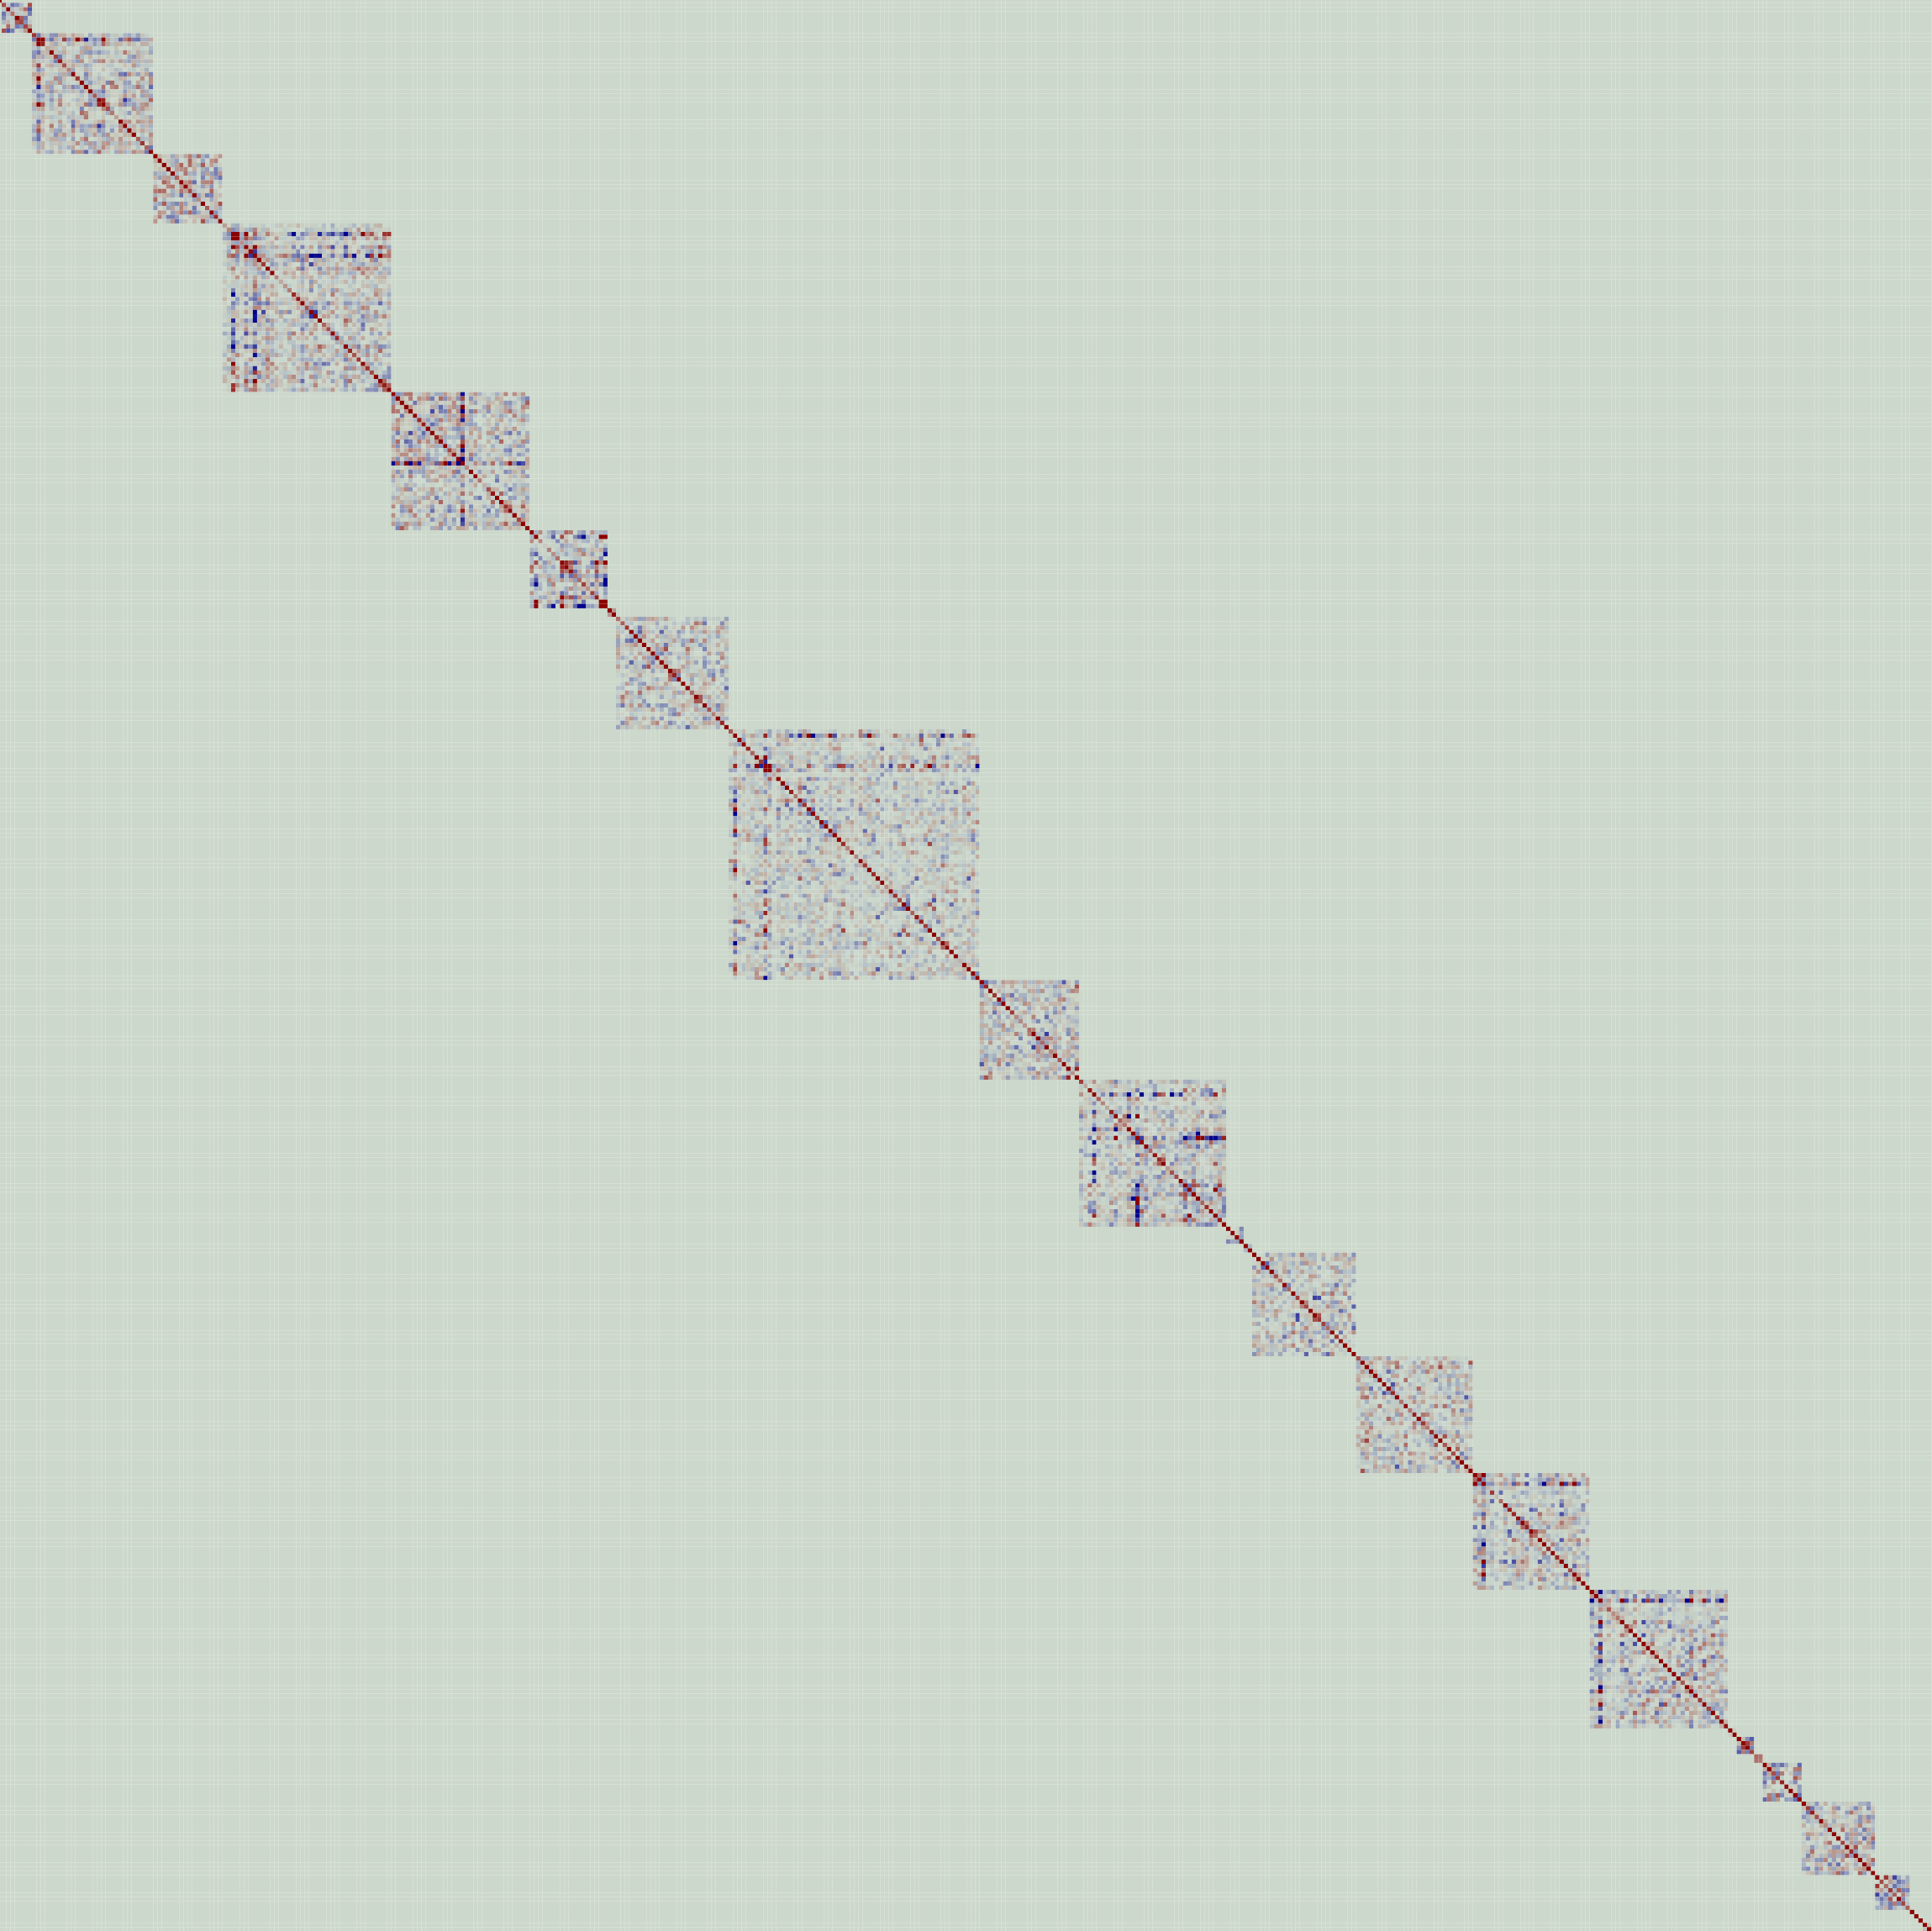
\includegraphics[height=\textheight]{AutF5_blocks.png}
\vfill
\end{center}
\end{frame}

\begin{frame}
\centering
\begin{tikzpicture}[scale=0.9]
\draw [thin, draw=black!20, fill=blue!5] (0,0) grid (10.18,-10.18) rectangle (0,0);
\node at (6.5, -9.5) {Original sdp constraint ($4\, 641 \times 4\, 641$)};
\node (ssdp) at (.5,-.5) {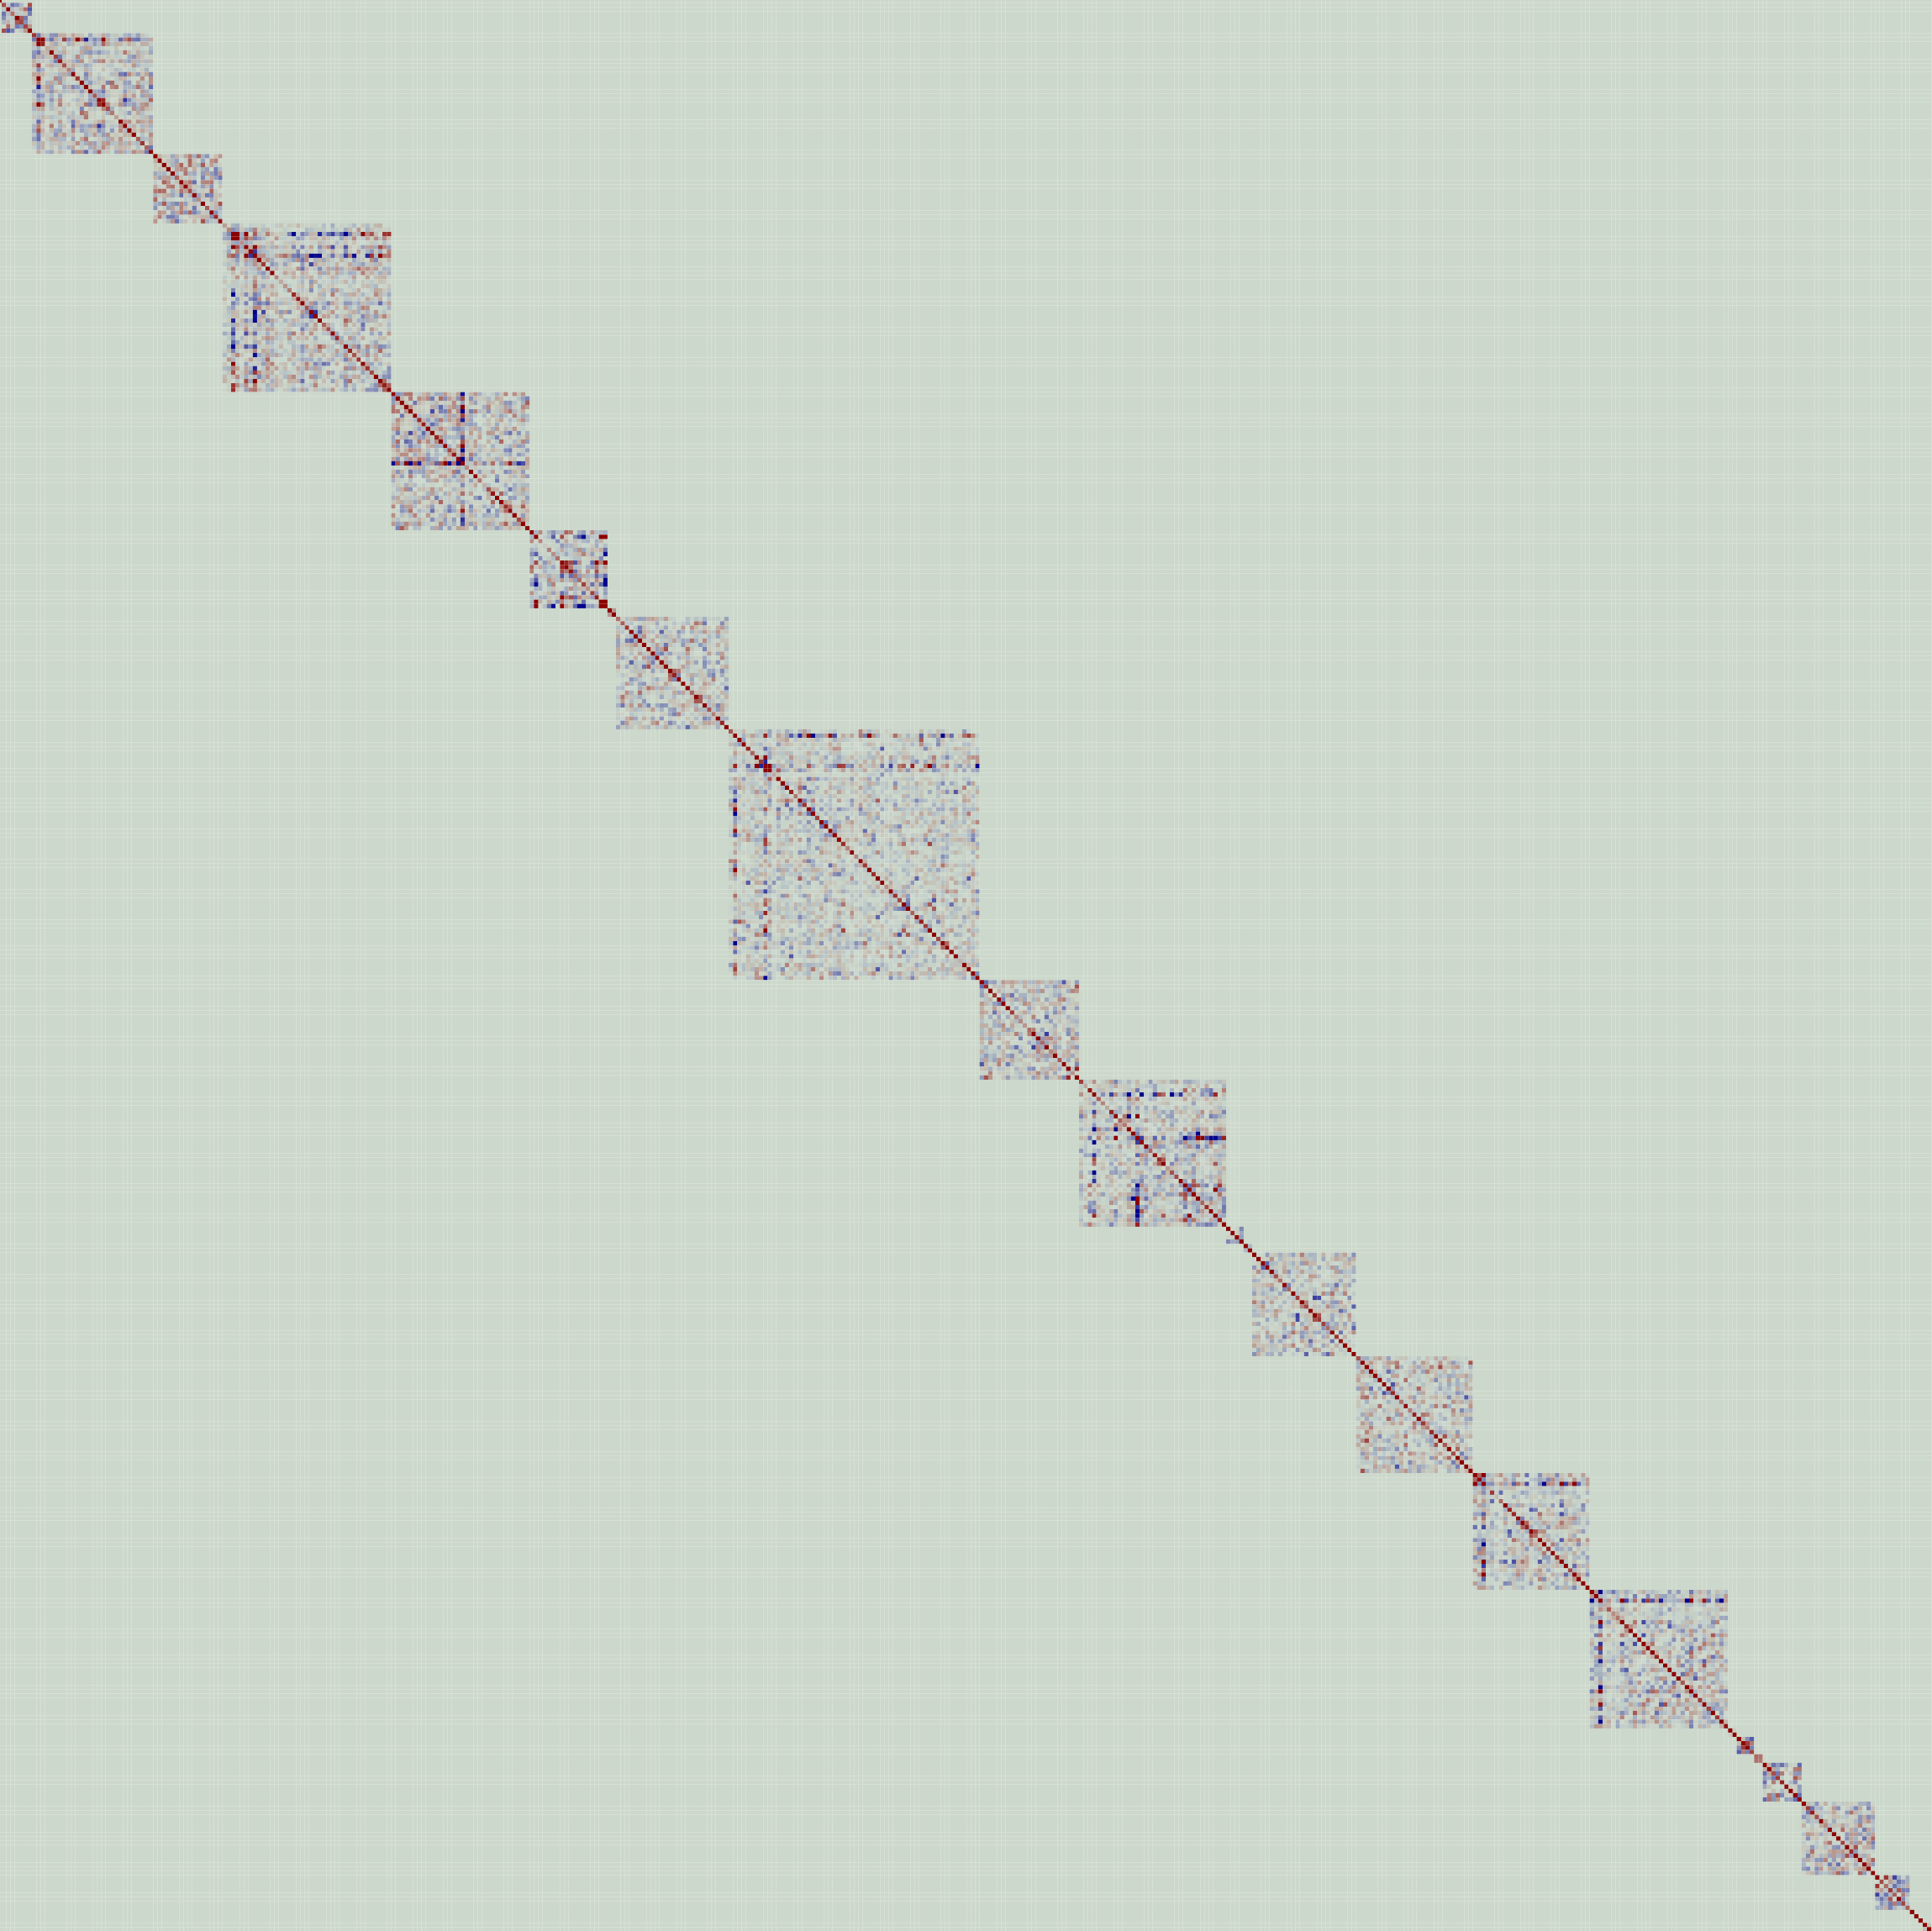
\includegraphics[width=0.9cm]{AutF5_blocks.png}};
\node (label) at (6.5,-.5) {Symmetrized sdp constraint ($448\times 448$)};
\draw [->] (label.west) -- (ssdp.east);
\end{tikzpicture}


\end{frame}






\end{document}
